\section{How the Shift Breaks the Classifier}
\label{sec:results-diagnosis}

\subsection{Over all pairs, the bias gain follows the predicted-marginal shift}
\label{sec:results-all-pairs}

Figure~\ref{fig:all-pairs} places each of the 21 shifted source--target pairs by the shift of its predicted-label
distribution, which needs no target labels, and by the macro-F1 that a bias correction adds to source TS. With
label-free batch calibration the gain rises with the predicted-marginal shift (Spearman $\rho = 0.687$,
$t(19) = 4.12$, permutation $p = 0.0008$), and it does so with MAP BCTS fitted on 50 labels as well ($\rho = 0.490$,
$t(19) = 2.45$, $p = 0.026$). Pairs that share a target corpus are not independent, so we repeat the analysis on the
mean gain of each of the 11 target corpora: $\rho = 0.773$ ($t(9) = 3.65$, $p = 0.007$) for batch calibration and
$\rho = 0.500$ ($t(9) = 1.73$, $p = 0.121$) for MAP BCTS. The gain is not a reward for a preserved ranking: across pairs
it is negatively associated with AUROC retention ($\rho = -0.471$, $t(19) = -2.33$, $p = 0.032$), because the pairs
with the largest marginal shifts also lose some ranking. Shrinkage TS changes no predicted class, so its macro-F1 gain
is exactly zero in every run.

\begin{figure}[t]
\centering
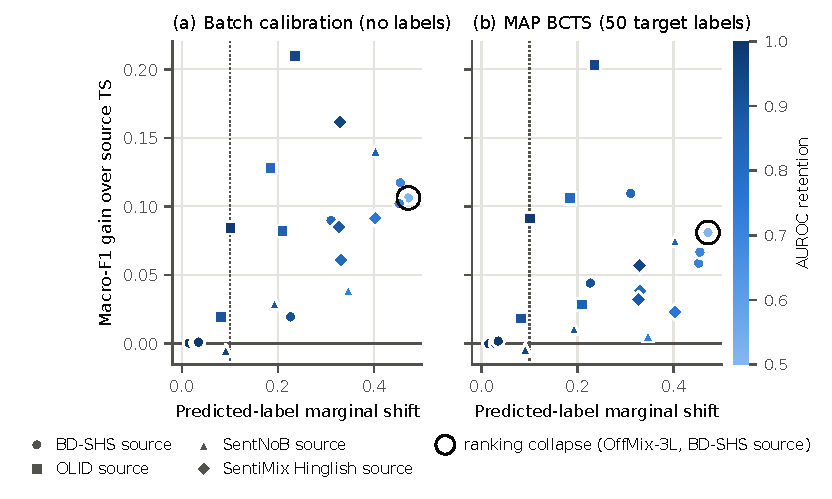
\includegraphics[width=\linewidth]{all_pairs_bias_gain.pdf}
\Description{Two scatter plots of macro-F1 gain against the shift of the predicted-label distribution for 21 source-target pairs; the gain rises with the shift for both bias corrections.}
\caption{Macro-F1 gain over source TS of a bias correction for the 21 shifted source--target pairs (means over the
converged runs of each source task). Horizontal: total-variation shift of the predicted-label distribution, computed
without target labels; dotted line at 0.10. Colour: AUROC retention. Marker shape: source task. (a) Label-free batch
calibration. (b) MAP BCTS with 50 target labels. The circled pair is the one ranking collapse.}
\label{fig:all-pairs}
\end{figure}

The descriptive regimes summarise the same picture. Encoders trained on BD-SHS keep their ranking on the Barishal and
Noakhali dialects (retention 0.994 and 0.990, marginal shift at most 0.035), and SentNoB encoders keep 0.957 of their
ranking on Sylheti; no correction improves on source TS there by more than 0.0035 nats, and spending 50 labels on the
temperature makes NLL slightly worse (0.450 against 0.442). For Sylheti this reading depends on the reference labels.
On the 72 test items on which the two authors' blind reading agreed, batch calibration raises NLL by 0.047 nats against
the SentNoB gold labels but lowers it by 0.045 against the authors' consensus, with opposite signs in every one of the
50 runs. ``No correction needed'' therefore holds against the gold labels, not against an independent reading of the
same translations. Two pairs show a finite temperature change with stable predicted proportions: the Chittagong
dialect ($\log T^{*}_{Q}/T_{P} = 0.297$, marginal shift 0.029) and BD-SHS as a target of the OLID-trained models
(0.407 and 0.082). Twelve pairs, from all four source tasks, keep a usable ranking (retention 0.70--0.98) while their
predicted marginal moves by 0.10--0.46: natural Banglish, Bangla-script code-mixing, MixTox-SA and English OLID for the
BD-SHS models; OffMix-3L, both scripts of Code-mixed Chaos and MixTox-SA for the OLID models; SentMix-3L and Hinglish
for the SentNoB models; and SentMix-3L and SentNoB for the Hinglish models. Spanglish keeps AUROC 0.609 and 0.648 for
the two sentiment sources but target TS is no better than a constant in most runs, as is Sylheti for the Hinglish
models. One pair collapses: BD-SHS models on OffMix-3L rank at AUROC 0.496 (0.387--0.589 across runs) with an
unbounded oracle temperature in every run. Where the operational thresholds are drawn moves these counts by a pair or
two (Appendix~\ref{sec:appendix-regime-sensitivity}), but not the conclusion that matters for practice: in each of the
16 pairs whose predicted marginal moves by more than 0.10, label-free bias correction raises macro-F1 in at least 93\%
of runs.

\subsection{Under a threshold shift, a temperature recovers log-loss but no decision}
\label{sec:results-threshold}

Table~\ref{tab:threshold-shift-operating-point} compares the corrections in the 12 threshold-shift pairs. Shrinkage
TS with 50 target labels lowers NLL from 0.892 to 0.728 but leaves macro-F1 at 0.527, as it must. Of the largest NLL
gain that any correction achieves, the temperature alone recovers 0.790 when units are weighted equally and 0.710 when
target corpora are: most of the log-loss, but none of the decisions. Every correction that moves the boundary changes
the decisions: batch calibration raises macro-F1 to 0.620, the MAP bias to 0.601 and MAP BCTS to 0.594, which also has
the lowest NLL among the deployable corrections (0.684). Weighting corpora equally lowers every value but keeps the
order of the methods (source TS 0.505, batch calibration 0.615, MAP BCTS 0.578); batch calibration then also has the
lower NLL (0.725 against 0.732).

\begin{table}[t]
\centering
\small
\caption{Corrections under threshold shift (R2: 12 source--target pairs, 7 target corpora, 386 run $\times$ pair units). F1 is macro-F1 on the target test split. Runs: mean over units; corpora: mean over corpora of the pair means. Labels: target labels used (50 calibration labels, 20 resamples). The last three rows are references, not deployable corrections: the true prior is the target calibration prior, the oracle bias is fitted on all target calibration labels, and the oracle threshold is tuned on the test labels themselves. Batch calibration uses the unlabelled target calibration split.}
\label{tab:threshold-shift-operating-point}
\resizebox{\textwidth}{!}{%
\begin{tabular}{lllrrrr}
\toprule
Correction & Adjusts & Labels & F1 (runs) & F1 (corpora) & NLL (runs) & NLL (corpora) \\
\midrule
Source TS & -- & 0 & 0.527 & 0.505 & 0.892 & 0.883 \\
Shrinkage TS & temperature & 50 & 0.527 & 0.505 & 0.728 & 0.771 \\
Prior adjustment, prior from labels & class prior & 50 & 0.531 & 0.524 & 0.918 & 0.882 \\
MAP bias & bias & 50 & 0.601 & 0.584 & 0.698 & 0.744 \\
MAP BCTS & temperature + bias & 50 & 0.594 & 0.578 & 0.684 & 0.732 \\
Batch calibration & bias & 0 & 0.620 & 0.615 & 0.699 & 0.725 \\
Tuned threshold & threshold & 50 & 0.631 & 0.618 & 0.713 & 0.749 \\
\midrule
Prior adjustment, true prior & class prior & prior & 0.536 & 0.531 & 0.902 & 0.864 \\
Oracle bias & bias & all & 0.626 & 0.609 & 0.665 & 0.701 \\
Oracle threshold & threshold & test & 0.660 & 0.649 & 0.693 & 0.726 \\
\bottomrule
\end{tabular}
}
\end{table}


A tuned threshold, the most direct correction of a decision, reaches 0.631 with 50 labels but has a worse NLL than the
bias corrections (0.713), and the oracle threshold tuned on the test labels themselves bounds what any correction of
this score can reach (0.660). Batch calibration is nearly as good as the NLL-optimal bias fitted on all target
calibration labels (0.620 against 0.626), so the remaining gap of the 50-label methods is an estimation problem, which
Section~\ref{sec:results-few-labels} locates. Training-time remedies that act like a temperature behave like one:
focal loss and label smoothing lower the uncalibrated ECE and NLL on most shifted conditions, but after source TS
neither is significantly better than cross-entropy on any condition, and label smoothing is significantly worse on
four of the five shifted offensive conditions (Appendix~\ref{sec:appendix-objectives}).

\subsection{The measured temperature change is mostly a misplaced bias}
\label{sec:results-decomposition}

If Proposition~\ref{prop:location} described these shifts exactly, a temperature fitted alone would rise to hedge the
misplaced threshold, while a temperature fitted jointly with a bias would stay at its source value. Fitting BCTS on all
target calibration labels of every run shows that this is what happens (Figure~\ref{fig:bcts-coordinates}). In the
threshold-shift pairs the mean change of $\log T$ is 0.976 when the temperature is fitted alone but 0.028 when it is
fitted with a bias (medians 0.989 and 0.069), and the bias alone recovers 0.932 of the BCTS log-loss gain, against
0.624 for the temperature alone. Two examples show the size of the effect: for the BD-SHS models on Bangla-script Chaos
the temperature-only change is 0.972 and the joint change $-0.075$, and for the OLID models on Banglish 1.185 and 0.078.
The temperature change survives the joint fit only where the descriptive labels say it should: on the Chittagong
dialect (0.323 alone, 0.258 jointly) and on the OffMix-3L collapse (2.461 and 2.212). The OLID models on BD-SHS, labelled
a temperature shift, sit in between (0.407 and 0.195), so part of their apparent temperature shift is also a bias.

\begin{figure}[t]
\centering
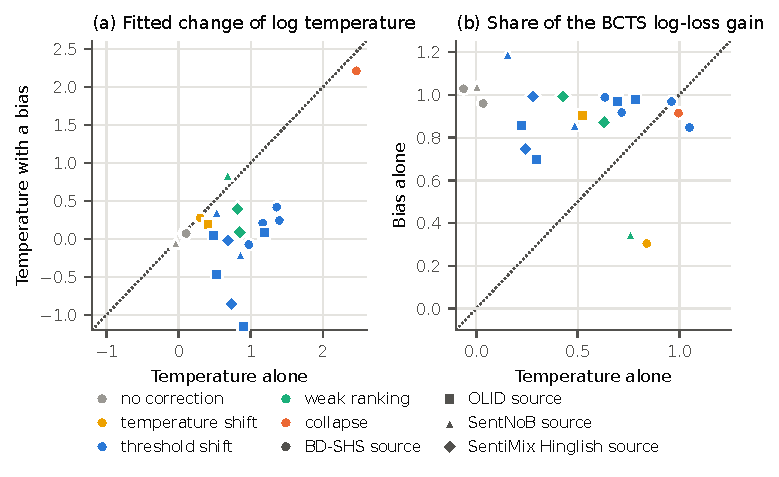
\includegraphics[width=\linewidth]{bcts_shift_coordinates.pdf}
\Description{Two scatter plots. Left: change of log temperature fitted alone against fitted jointly with a bias; threshold-shift pairs lie far below the diagonal near zero. Right: share of the log-loss gain recovered by temperature alone against bias alone; most pairs lie above the diagonal near one.}
\caption{Temperature against bias in the 21 shifted pairs (means over runs; BCTS fitted on all target calibration
labels). (a) Change of $\log T$ when the temperature is fitted alone (horizontal) and jointly with a bias (vertical);
points far below the dotted diagonal are temperature changes that a bias explains. (b) Share of the BCTS log-loss gain
recovered by the temperature alone and by the bias alone. Colour: descriptive regime; marker shape: source task.}
\label{fig:bcts-coordinates}
\end{figure}

The bias is not a change of the class prior. In the threshold-shift pairs, a prior adjustment with the true target
prior lifts macro-F1 only from 0.527 to 0.536 (Table~\ref{tab:threshold-shift-operating-point}), against 0.626 for the
oracle bias: the prior change explains almost none of the required move, and the rest is a shift of the score itself,
the $\delta$ of Proposition~\ref{prop:location}. Label-shift estimators assume that the score does not move, so they
should fail on these targets, and they do. Black-box shift estimation \citep{lipton2018bbse} and maximum-likelihood
label shift \citep{saerens2002adjusting, alexandari2020maximum} on TS and on BCTS posteriors estimate the target prior
with a total-variation error of 0.297--0.480 on the five BD-SHS-source targets beyond the dialects, whose true prior
moves by only 0.001--0.149 from the source, and they lower macro-F1 below source TS on every pair whose predicted
marginal moves by more than 0.10. On Banglish, for instance, macro-F1 falls from 0.577 to 0.450, 0.411 and 0.392, while
batch calibration reaches 0.666. Even where the prior really changes, for OLID models on BD-SHS (total variation
0.149), none of the three estimators recovers it (errors 0.153, 0.220 and 0.187), whereas the true prior would raise
macro-F1 from 0.681 to 0.699. The failure of these estimators is a symptom: the label-shift assumption does not hold
for dialect, script and code-mixing shift.

\subsection{What 50 labels can and cannot fix}
\label{sec:results-few-labels}

MAP BCTS trails batch calibration in macro-F1 although it uses labels. Projecting the bias that each method fits from
50 labels onto the oracle bias, with 1 meaning the full move, locates the shortfall. On the offensive targets the
maximum-likelihood bias reaches a median of 0.960 of the move and the MAP bias 0.873; on the sentiment targets the
maximum-likelihood bias reaches 0.980 but the MAP bias only 0.314 and the bias of MAP BCTS 0.187, against 0.639 for the
bias implied by batch calibration. The sentiment prior variance for the bias is estimated from the offensive task and
is small, so it holds the sentiment bias near its source value. The labels are informative; the prior, not the label
budget, is why MAP BCTS falls behind on the threshold-shift pairs.

Batch calibration has its own assumption: it pulls the predicted proportions towards uniform. Resampling every target
of the two offensive source tasks to a fixed positive share $\pi_+$ shows when this backfires
(Table~\ref{tab:prior-shift-ablation} in the appendix). At $\pi_+ = 0.1$, the typical situation in content moderation,
batch calibration lowers macro-F1 to 0.631 from 0.654 with source TS and raises NLL from 0.31 to 0.56; a class prior
estimated from 50 labels repairs the rare-positive case on average (0.661 and 0.27), as does MAP BCTS (0.665 and
0.25), although both stay worse than source TS in 30\% and 46\% of units on macro-F1. Every correction fitted on
target items also inherits their prior. When the 50 labels and the unlabelled batch come from a target with
$\pi_+ = 0.9$ and the deployment stream has $\pi_+ = 0.1$, MAP BCTS falls to macro-F1 0.252 and is better than source
TS (0.651) in none of the units, the label-estimated prior reaches 0.421, and batch calibration, whose uniform target
does not depend on the batch prior, reaches 0.680. In the reverse direction (0.1 to 0.9) the four give 0.434, 0.359,
0.404 and 0.575 in the same order of source TS, MAP BCTS, label-estimated prior and batch calibration. With matched
priors at 0.5 MAP BCTS is the best of them (0.713). The few-label recipe therefore assumes that the labelled items come
from the deployment distribution, and a correction must be refitted when the prior drifts.

\subsection{Robustness}
\label{sec:results-robustness}

The 12 threshold-shift pairs rest on seven target corpora. In every one of them batch calibration raises the mean
macro-F1 (exact two-sided sign test, 7 of 7, $p = 0.0156$), and the same holds for the nine corpora of the 16 pairs
with a predicted-marginal shift above 0.10 (9 of 9, $p = 0.0039$). Without the two student-written corpora, OffMix-3L
and SentMix-3L, five corpora remain and five of five are positive, which gives $p = 0.0625$, the smallest value a
two-sided sign test can reach with five units; the corpus-weighted gain is 0.081 with a hierarchical bootstrap 95\%
interval of 0.052--0.105. On the natural corpora of the pairs with a marginal shift above 0.10, 7 of 7 are positive
($p = 0.0156$; gain 0.076, interval 0.055--0.096). A mixed model with random intercepts for corpus and for pair within
corpus gives a threshold-shift gain of 0.108 (standard error 0.020, $z = 5.38$, 95\% interval 0.069--0.147) and, over
all 21 pairs, a slope of 0.219 on the predicted-marginal shift ($z = 2.31$, $p = 0.021$;
Appendix~\ref{sec:appendix-mixed}). Seven purposively chosen corpora cannot support a claim about a population of
corpora; these checks show that the effect is not carried by one corpus or one weighting.
